\section{组合投资理论}
\begin{enumerate}
    \item 投资组合的标准差一定小于每一项构成资产的标准差吗?为什么?\\
    \sol\\
    不一定。根据式(2-7),$\displaystyle \sigma^2(R_p)=\sum\limits_{i=1}^N \sum\limits_{j=1}^N x_ix_j\sigma_{ij}=\sum\limits_{i=1}^N \sum\limits_{j=1}^N x_ix_j \rho_{ij} \sigma_i \sigma_j$,显然这与$x_i,x_j,\rho_{ij},\sigma_i,\sigma_j$都有关。\\
    或者举个例子,假设两种股票$\sigma_1=0.2,\sigma_2=0.4$,相关系数为1,$X=(0.5,0.5)^{\mathrm{T}}$,则$\sigma(R_p)=0.5 \times 0.2 + 0.5 \times 0.4=0.3 > 0.2$。
    \item 什么是资本市场上投资者对于股票投资收益的同质预期,这一假设对于资产配置分析起到什么作用?\\
    \sol\\
    同质预期:所有投资机会的期望收益值和方差(协方差)均有相同的估计,是资本资产定价模型(CAPM模型)的模型假设之一。\\
    作用:为资产配置分析提供了新的模型,在均值-方差模型的基础上拓展出了资本资产定价模型。
    \item 什么是资产配置?马科维茨均值-方差模型怎样适合资产配置活动的?\\
    \sol\\
    资产配置:根据投资需求将投资资金在不同资产类别之间进行分配,通常是将资产在低风险、低收益证券与高风险、高收益证券之间进行分配。\\
    均值-方差模型的基本假设是投资者从根本上讲都是回避风险的,这一假定意味着投资者若接受高风险的话,则必定要有高回报率来补偿。所以,如果在具有相同回报率的两个证券之间进行选择的话,则任何投资者都将会选择风险较小的,从而舍弃风险较大的,这一假定意味着投资者要使期望效用最大化,而不仅仅是使期望的回报率最大化。
    \item 若一投资组合包含$A$、$B$两种股票,股票$A$的期望收益率为14\%,标准差为10\%;股票$B$的期望收益率为18\%,标准差为16\%,两种股票的相关系数为0.4,投资股票$A$的权重为40\%,$B$的权重为60\%,则该投资组合的期望收益率与标准差分别是多少?\\
    \sol
    \begin{align*}
        E(R_p) & = 0.4 \times 14\% + 0.6 \times 18\% = 16.4\%,\\
        \sigma(R_p) & = \sqrt{0.4^2 \times (10\%)^2 + 2\times 0.4 \times 0.6 \times 0.4 \times 10\% \times 16\% + 0.6^2 \times (16\%)^2} = 11.78 \%.
    \end{align*}
    \item 某企业有甲、乙两个独立性投资项目,计划投资额均为1000万元,其收益率的概率分布如下表所示,计算两个项目的期望收益率、标准差,以及投资组合的期望收益率和标准差。
    \begin{center}
        \setlength{\tabcolsep}{14mm}{
        \begin{tabular}{c|c|c|c}
            \hline
            市场状况 & 概率 & 甲项目/\% & 乙项目/\% \\ \hline
            好 & 0.3 & 20 & 30 \\ \hline
            一般 & 0.5 & 10 & 10 \\ \hline
            差 & 0.2 & 5 & $-5$ \\ \hline
        \end{tabular}}
    \end{center}
    \sol
    \[\begin{cases}
        E(\text{甲}) = 12\%, \\ \displaystyle\sigma(\text{甲}) = \frac{\sqrt{31}}{100} \approx 5.6\%
    \end{cases},
    \begin{cases}
        E(\text{乙}) = 13\%, \\ \displaystyle\sigma(\text{乙}) = \frac{\sqrt{39}}{50} \approx 12.5\%
    \end{cases}\]
    由于甲、乙是独立的且投资数额相同,所以其相关系数为0,权重均为50\%,则
    \begin{align*}
        E(R_p) & = 0.5 \times 12\% + 0.5 \times 13\% = 12.5\%,\\
        \sigma(R_p) & = \sqrt{0.5^2 \times (5.6\%)^2 + 2 \times 0.5 \times 0.5 \times 0 \times 5.6\% \times 12.5\% + 0.5^2 \times (12.5\%)^2} = \frac{\sqrt{187}}{200} \approx 6.8 \%.
    \end{align*}
    \item 投资组合中有两只构成股票,股票$A$的期望收益率为15\%,标准差为20\%,股票$B$的期望收益率为20\%,标准差为25\%。如果两只股票的相关系数为0.3,制作使用两只股票进行组合的可能组合曲线。如果相关系数变为$-0.3$,再次制作曲线,并进行比较。\\
    \sol\\
    可以计算得到两种情况下,投资组合的期望收益率和标准差
    \begin{center}
        \setlength{\tabcolsep}{9mm}{
        \begin{tabular}{c|c|c|c|c|c}
            \hline
            \multicolumn{3}{c|}{$\rho = 0.3$} & \multicolumn{3}{|c}{$\rho = -0.3$} \\ \hline
            $\alpha$ & $E(R_p)$ & $\sigma(R_p)$ & $\alpha$ & $E(R_p)$ & $\sigma(R_p)$ \\ \hline
            $-0.5$ & 22.5\% & 35.8\% & $-0.5$ & 22.5\% & 41.6\% \\ \hline
            $0$ & 20\% & 25\% & $0$ & 20\% & 25\% \\ \hline
            $0.25$ & 18.75\% & 20.8\% & $0.25$ & 18.75\% & 17.9\% \\ \hline
            $0.5$ & 17.5\% & 18.2\% & $0.5$ & 17.5\% & 13.5\% \\ \hline
            $1$ & 15\% & 20\% & $1$ & 15\% & 20\% \\ \hline
            $1.5$ & 12.5\% & 28.8\% & $1.5$ & 12.5\% & 35.8\% \\ \hline
        \end{tabular}}
    \end{center}
    曲线如下:
    \begin{center}
        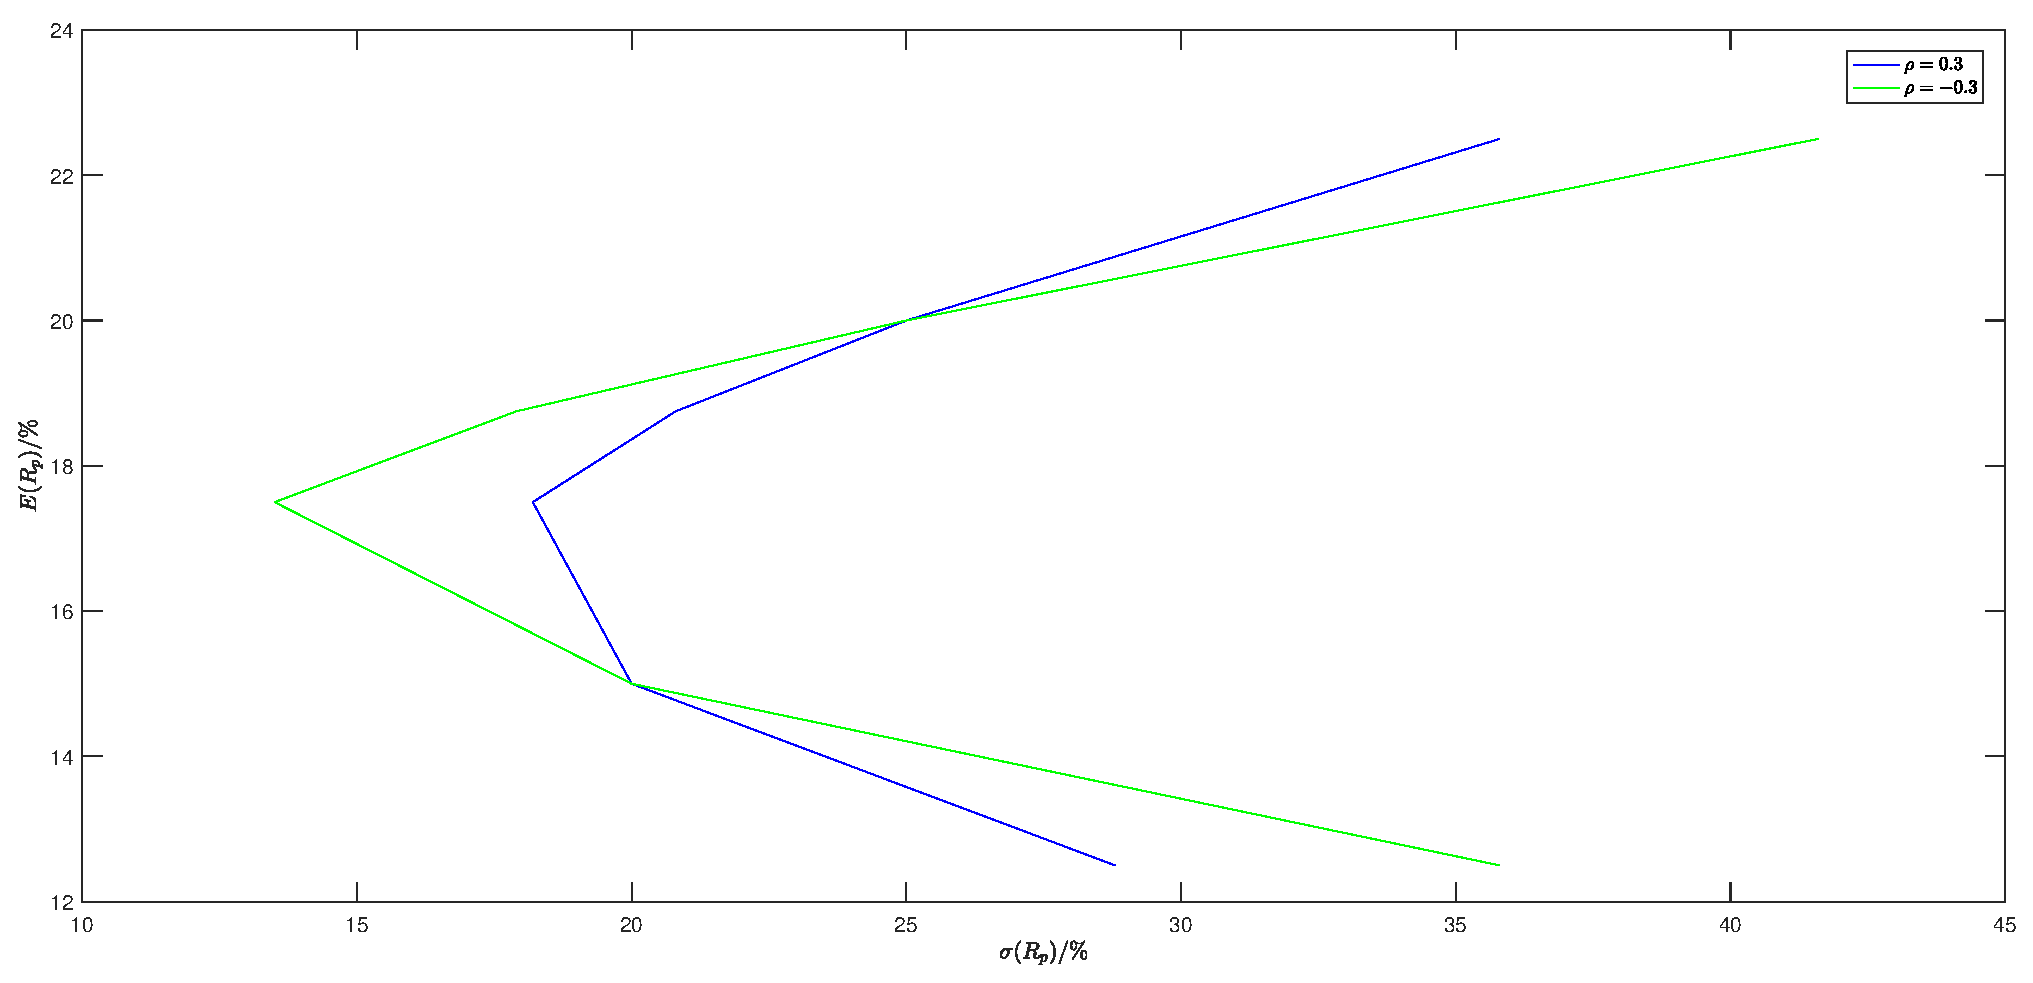
\includegraphics[scale=0.49]{2_6.eps}
    \end{center}
    比较:$\rho = -0.3$比$\rho = 0.3$凸得更厉害。\\
    Matlab绘图命令如下:
\begin{lstlisting}
y = [22.5, 20, 18.75, 17.5, 15, 12.5];
x1 = [35.8, 25, 20.8, 18.2, 20, 28.8];
x2 = [41.6, 25, 17.9, 13.5, 20, 35.8];
plot(x1, y, 'b');
hold on;
plot(x2, y, 'g');
\end{lstlisting}
% xlabel('$\sigma(R_p)/\%$', 'interpreter', 'latex');
% ylabel('$E(R_p)/\%$', 'interpreter', 'latex');
% l = legend('$\rho = 0.3$', '$\rho = -0.3$');
% set(l, 'Interpreter', 'latex');
    \item 依据下表求均方效率边界,至少得到10个点,并画图。\textcolor{red}{(注意下表的划分与书本不同,书本有误)}
    \begin{center}
        \setlength{\tabcolsep}{7mm}{
        \begin{tabular}{c|c|c|c|c|c|c}
            \hline
            证券 & \multicolumn{5}{|c|}{协方差/\%} & 收益率/\% \\ \hline
            1 & 2.30 & 0.93 & 0.62 & 0.74 & $-0.23$ & 15.10 \\ \hline
            2 & 0.93 & 1.40 & 0.22 & 0.56 & 0.26 & 12.50 \\ \hline
            3 & 0.62 & 0.22 & 1.80 & 0.78 & $-0.27$ & 14.70 \\ \hline
            4 & 0.74 & 0.56 & 0.78 & 3.40 & $-0.56$ & 9.02 \\ \hline
            5 & $-0.23$ & 0.26 & $-0.27$ & $-0.56$ & 2.60 & 17.68 \\ \hline
        \end{tabular}}
    \end{center}
    \sol\\
    图如下:
    \begin{center}
        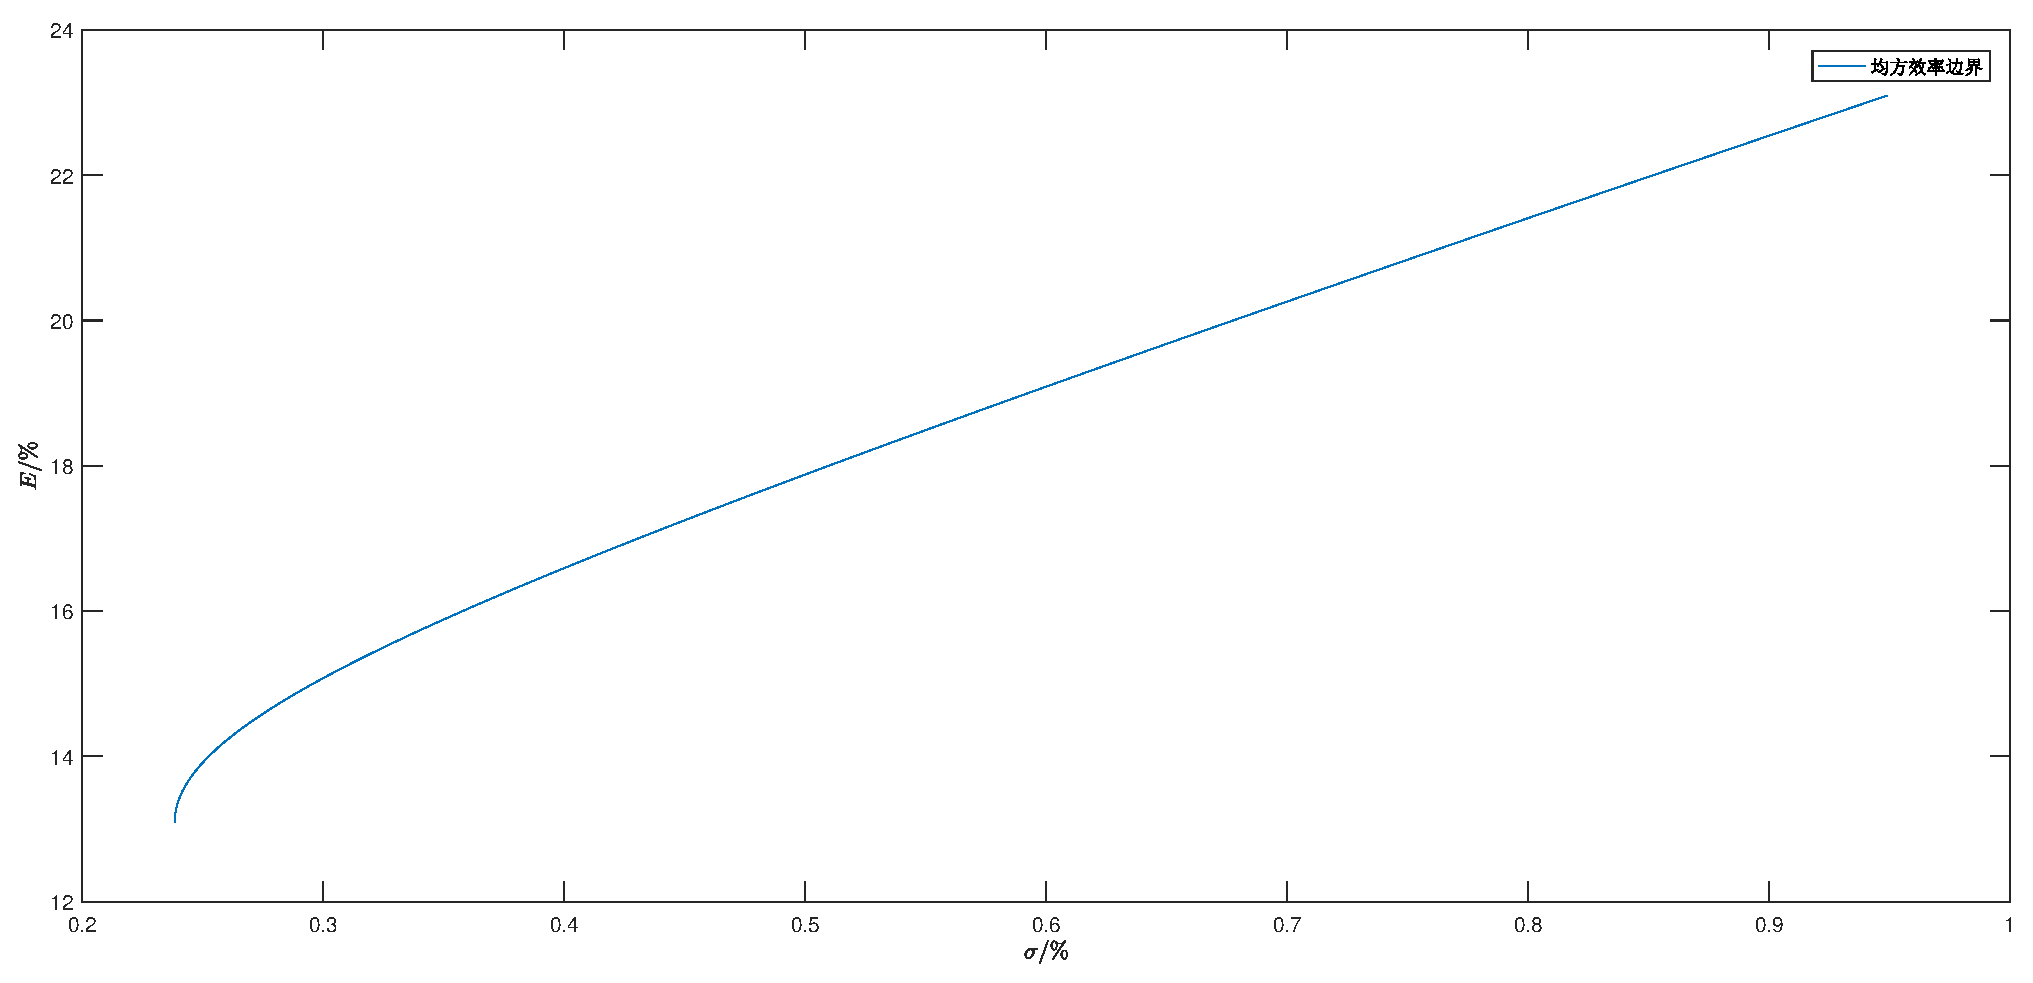
\includegraphics[scale=0.49]{2_7.eps}
    \end{center}
    Matlab绘图命令如下:
\begin{lstlisting}
S = [2.3, 0.93, 0.62, 0.74, -0.23; 0.93, 1.40, 0.22, 0.56, 0.26; 0.62, 0.22, 1.8, 0.78, -0.27; 0.74, 0.56, 0.78, 3.4, -0.56; -0.23, 0.26, -0.27, -0.56, 2.6];
r = [15.1; 12.5; 14.7; 9.02; 17.68];
a = r' * S * r;
b = ones(1, 5) * S * r;
c = ones(1, 5) * S * ones(5, 1);
d = a * c - b ^ 2;
y = b / c : 0.01 : b / c + 10;
x = sqrt(c / d * (y - b / c) .^ 2 + 1 / c);
plot(x, y);
legend('均方效率边界');
\end{lstlisting}
% xlabel('$\sigma/\%$', 'interpreter', 'latex');
% ylabel('$E/\%$', 'interpreter', 'latex');
    \item 三个证券的期望收益率、收益标准差和相关系数见下表:
    \begin{center}
        \setlength{\tabcolsep}{14mm}{
        \begin{tabular}{c|c|c|c}
            \hline
            证券 & 预期收益率 & 标准差 & 相关系数 \\ \hline
            A & 0.08 & 0.20 & 0.18 \\ \hline
            B & 0.12 & 0.25 & 0.20 \\ \hline
            C & 0.15 & 0.15 & $-0.15$ \\ \hline
        \end{tabular}}
    \end{center}
    求绝对最小方差资产组合的期望收益率和标准差,该资产组合系数是多少?\\
    \sol
    \[{\small V = \begin{pmatrix}
        0.2^2 & 0.2 \times 0.25 \times (-0.15) & 0.2 \times 0.15 \times 0.2\\
        0.2 \times 0.25 \times (-0.15) & 0.25^2 & 0.25 \times 0.15 \times 0.18\\
        0.2 \times 0.15 \times 0.2 & 0.25 \times 0.15 \times 0.18 & 0.15^2
    \end{pmatrix}=\begin{pmatrix}
        0.04 & -0.0075 & 0.006 \\ -0.0075 & 0.0625 & 0.00675\\ 0.006 & 0.00675 & 0.0225
    \end{pmatrix}}\]
    则
    \[X=\frac{V^{-1}i}{i'V^{-1}i}=(0.3174,0.2103,0.4723)^{\mathrm{T}}.\]
    则向A证券投资31.74\%,向B证券投资21.03\%,向C证券投资47.23\%。
    \begin{align*}
        E(R_p) & = 0.3174 \times 0.08 + 0.2103 \times 0.12 + 0.4723 \times 0.15 = 0.121473,\\
        \sigma^2(R_p) & = 0.3174^2 \times 0.2^2 + 0.2103^2 \times 0.25^2 + 0.4723^2 \times 0.15^2\\
        & + 2 \times 0.3174 \times 0.2103 \times (-0.15) \times 0.2 \times 0.25\\
        & + 2 \times 0.3174 \times 0.4723 \times 0.2 \times 0.2 \times 0.15\\
        & + 2 \times 0.2103 \times 0.4723 \times 0.18 \times 0.25 \times 0.15 = 0.01435,\\
        \sigma(R_p) & = 0.1198.
    \end{align*}
    \item 对于上题中的三个证券构成的资产组合,假设其期望收益为18\%,在所有有效资产组合中,计算方差最小的资产组合。\\
    \sol\\
    由上题可知,
    \begin{align*}
        & A = \begin{pmatrix}
            0.08 & 0.12 & 0.15\\1 & 1 & 1
        \end{pmatrix}V^{-1}\begin{pmatrix}
            0.08 & 1\\0.12 & 1\\0.15 & 1
        \end{pmatrix},\\
        & X=V^{-1}\begin{pmatrix}
            0.08 & 1\\0.12 & 1\\0.15 & 1
        \end{pmatrix}A^{-1}\begin{pmatrix}
            0.18\\1
        \end{pmatrix}=(-0.4306,0.0047,1.4259)^{\mathrm{T}}.
    \end{align*}
    则向A证券投资$-43.06\%$,向B证券投资0.47\%,向C证券投资142.59\%。
    \item 假设市场证券组合的期望收益为23\%,市场利率为7\%。市场证券组合的标准差为32\%。假设市场是有效的,请给出资本市场线的方程。考虑一个期望收益为39\%的有效边界上的资产组合,计算该资产组合的标准差。如用1000元进行投资,该如何投资才能得到收益?若投资300元用于无风险证券,700元用于市场证券组合,那么年底的收益为多少?\\
    \sol\\
    由题知:$i=0.07,r_m=0.23,\sigma_m=0.32$,则
    \[r=0.07+\frac{0.23-0.07}{0.32}\sigma=0.07+0.5\sigma,\]
    故资本市场线方程为$r=0.07+0.5\sigma.$\\
    取$r=0.39$,则
    \[0.39=0.07+0.5\sigma \Rightarrow \sigma = 0.64,\]
    故该资产组合的标准差$\sigma = 0.64.$\\
    设1000元中$x$元用于市场证券组合,$1000-x$元用于无风险证券,而本题无风险证券的期望收益为7\%,标准差为0,由于要得到收益,即期望收益要达到0,则
    \[E(R_p) = \frac{x}{1000} \times 0.23 + \frac{1000-x}{1000} \times 0.07 = 0 \Rightarrow x = -437.5.\]
    故用1000元,无论如何投资,都能得到收益。\\
    若投资300元用于无风险证券,700元用于市场证券组合,则
    \[E(R_p) = 0.3 \times 0.23 + 0.7 \times 0.07 = 0.118 \Rightarrow R_p = 0.118 \times 1000 = 118.\]
    故年底的收益为118元。
\end{enumerate}
\clearpage